% BotRepel whitepaper. Build with `bun run whitepaper` (needs Tectonic); the PDF is written next to this file.
\documentclass[11pt]{article}

\usepackage[margin=1.1in]{geometry}
\usepackage{amsmath,amssymb}
\usepackage{booktabs,tabularx}
\usepackage{microtype}
\usepackage{enumitem}
\usepackage{xcolor}
\usepackage{float}
\usepackage{tikz}
\usetikzlibrary{arrows.meta,positioning}
\usepackage[hidelinks]{hyperref}

\setlist{itemsep=2pt,topsep=4pt}
\renewcommand{\arraystretch}{1.2}
\newcolumntype{L}{>{\raggedright\arraybackslash}X}

\title{\textbf{Proof of a present human on the open web}\\[4pt]
  \large Risk-gated, layered verification with light-reflection liveness}
\author{BotRepel\\\small\url{https://botrepel.com}}
\date{October 2026}

\hypersetup{
  pdftitle={Proof of a present human on the open web},
  pdfauthor={BotRepel},
  pdfsubject={Human verification, liveness detection, bot defense}
}

\begin{document}
\maketitle

\begin{abstract}
CAPTCHAs no longer separate people from software. Vision models solve image puzzles, LLM browser
agents click through checkbox challenges, and solving farms sell the rest for about a tenth of a
cent each. At the other end of the market, identity verification proves far more than most sites
need and costs a hundred to a thousand times as much. We describe BotRepel, a verification
service that sits between the two. A passive risk tier decides who is challenged at all. Visitors
who are challenged step up to the cheapest proof the action requires: a passkey ceremony that
shows a person is present on a real device, or a two-second light-reflection liveness check that
shows a live face is in front of the screen right now. We state the threat model plainly. The
browser cannot attest its camera, so we do not claim to stop a funded, targeted attacker. We
claim to raise the per-session cost of passing from a fraction of a cent to building and running
a physically correct, real-time relighting injector, while storing no faces and matching no
identities.
\end{abstract}

\section{The problem}

Bot defense on the web has relied on tasks that were easy for people and hard for programs.
That gap has closed.

\begin{itemize}
  \item reCAPTCHA v2 image challenges have been solved at 100\% by an academic pipeline
        \cite{eth-recaptcha}, and general vision models solve 28--60\% of them unaided.
  \item Halligan solved 60.7\% across 26 CAPTCHA families \cite{halligan}.
  \item A commercial LLM browser agent clicked through Cloudflare's ``I am not a robot''
        checkbox in 2025 \cite{chatgpt-agent}.
  \item A vendor-run benchmark found that Turnstile caught none of three LLM browser agents,
        and hCaptcha caught 0--16\% \cite{poh-benchmark}.
\end{itemize}

Passive scoring alone fails for the same reason: an agent driving a real browser on a real
machine looks like a person. Proof-of-work only meters traffic, and the work is cheap for anyone
with a GPU.

Identity verification (IDV) does stop bots, but it answers a different question (\emph{who is
this?}) at a different price, roughly \$0.80--\$1.89 per check \cite{pricing}. It also collects
government documents and face templates, which carry breach risk and legal obligations that a
signup form does not need.

What most sites need is narrower: \emph{is a human present for this action, now?} Large
platforms reached the same conclusion in 2026. X checks only accounts flagged for automated
behavior and leads with on-device biometrics; Reddit checks ``fishy'' accounts with a passkey;
Discord never asks over 90\% of users \cite{x-liveness,reddit,discord}. Their shared pattern is
to challenge on risk and to lead with camera-free proof. BotRepel brings that pattern to any
website through one widget and one server-side call.

\section{Design overview}


BotRepel defines three ordered assurance levels,
\[
  \textsf{invisible} \prec \textsf{presence} \prec \textsf{liveness},
\]
and a token proving one level satisfies every level below it. A site sets a minimum level per
action, for example \textsf{invisible} for newsletter signup, \textsf{presence} for posting and
\textsf{liveness} for payouts. At challenge time the server computes
\begin{equation}
  \text{required}(a, r) = \max\bigl(\text{policy}(a),\; \ell(r)\bigr),\qquad
  \ell(r) =
  \begin{cases}
    \textsf{liveness} & r \ge 0.8\\
    \textsf{presence} & r \ge 0.5\\
    \textsf{invisible} & \text{otherwise}
  \end{cases}
  \label{eq:required}
\end{equation}
where $a$ is the action and $r \in [0,1]$ the visit's risk score. Policy sets a floor; risk can
only raise it.

\begin{figure}[H]
\centering
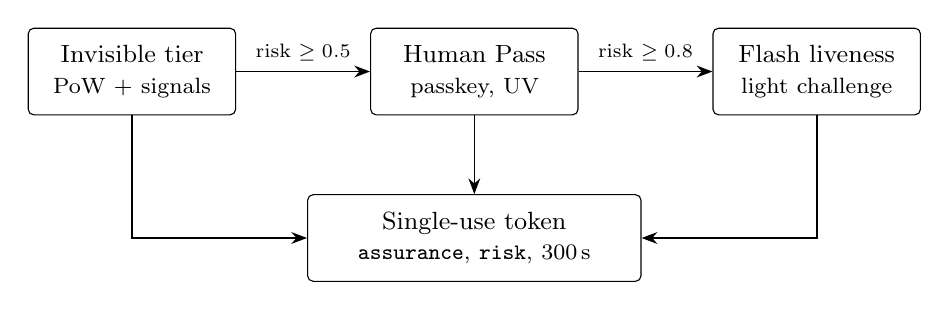
\begin{tikzpicture}[
  node distance=6mm and 17mm,
  box/.style={draw, rounded corners=2pt, align=center, font=\small, minimum height=11mm, text width=24mm},
  arr/.style={-{Stealth[length=2mm]}, semithick}]
  \node[box] (risk) {Invisible tier\\\footnotesize PoW + signals};
  \node[box, right=of risk] (pass) {Human Pass\\\footnotesize passkey, UV};
  \node[box, right=of pass] (flash) {Flash liveness\\\footnotesize light challenge};
  \node[box, below=10mm of pass, text width=40mm] (token) {Single-use token\\\footnotesize\texttt{assurance}, \texttt{risk}, 300\,s};
  \draw[arr] (risk) -- node[above, font=\scriptsize]{risk $\ge 0.5$} (pass);
  \draw[arr] (pass) -- node[above, font=\scriptsize]{risk $\ge 0.8$} (flash);
  \draw[arr] (risk) |- (token);
  \draw[arr] (pass) -- (token);
  \draw[arr] (flash) |- (token);
\end{tikzpicture}
\caption{The assurance ladder. A visit is served the strongest of the site's policy for the action
and the level its risk score demands. Every path ends in the same kind of token.}
\label{fig:ladder}
\end{figure}

The widget runs in a cross-origin iframe and returns an opaque token to the host page. The
site's backend redeems the token with its secret key (\texttt{siteverify}), which returns the
proven assurance, the action, the hostname and the risk score. Tokens are single-use and expire
after 300 seconds. Redemption is one atomic conditional update, so two concurrent verifications
of the same token cannot both succeed. The account is charged only on a successful redemption,
which means solving challenges cannot drain a customer's credit.

\section{The invisible tier}

\subsection{Proof-of-work as a meter}

Each challenge carries a fresh 22-character seed $s$ and a difficulty $b$. The client searches
for a decimal nonce $n$ such that $\mathrm{SHA\text{-}256}(s \,\|\, n)$ has at least $b$ leading
zero bits; the server checks the answer with a single hash. Difficulty grows with risk,
\begin{equation}
  b(r) = \min\bigl(21,\; 17 + \operatorname{round}(4r)\bigr),
\end{equation}
so the expected work, $2^{b}$ hashes, ranges from about $1.3 \times 10^5$ to $2.1 \times 10^6$.
At the 1{,}000--5{,}000 hashes per millisecond typical of browser JavaScript, a low-risk visitor
waits tens of milliseconds and a suspicious one up to about two seconds. Challenges expire after
120 seconds and are claimed atomically, so one solution mints at most one token.

We do not treat proof-of-work as evidence of humanity. Its job is to put a marginal cost on every
attempt and to give the server a timing measurement. Because the nonce counts up from zero, its
value is the number of attempts. Dividing by the reported solve time gives a hash rate, and a rate
above 20{,}000 hashes per millisecond, judged only once there are at least $10^4$ attempts, means
the work was done somewhere other than browser JavaScript.

\subsection{Risk scoring}

The widget reports a small, strictly validated set of browser signals. The server combines them
with its own observations into an additive score capped at 1 (Table~\ref{tab:risk}).

\begin{table}[H]
\centering
\small
\begin{tabularx}{\linewidth}{l r L}
  \toprule
  Signal & Weight & Meaning \\
  \midrule
  \texttt{webdriver} & 0.8 & The automation flag is set. \\
  \texttt{headless} & 0.6 & The user agent says headless or contradicts client hints. \\
  \texttt{cdp} & 0.4 & A DevTools-protocol client touched a stack getter during serialization. \\
  \texttt{zeroWindow} & 0.4 & Window metrics that only automation produces. \\
  offloaded work & 0.3 & Hash rate above any browser JavaScript engine. \\
  velocity & 0.3 & The IP exceeded 30 challenges per minute for this site. \\
  \bottomrule
\end{tabularx}
\caption{Risk signals and weights. Signals can only add risk.}
\label{tab:risk}
\end{table}

Two rules shape the score. First, a signal can only raise risk, never lower it. A bot controls
everything the client reports, so a report of ``looks human'' carries no information; a report of
``looks automated'' is a mistake no honest client makes. Second, no single weak signal crosses a
step-up threshold. A developer testing their own form has DevTools open, so \texttt{cdp} alone
scores 0.4, below the 0.5 line, while any second signal tips it over.

The score decides \emph{who is challenged}, never who passes. An agent that hides every signal
still faces the site's per-action policy floor.

\section{Human Pass}

A Human Pass is a WebAuthn passkey created once, after the person passes a liveness check, and
used afterwards with user verification: Face ID, a fingerprint, or a device PIN. A later
assertion proves that the same authenticator is present and that its owner unlocked it. For
\textsf{presence}, this is the cheapest strong proof the web platform offers: one tap, no camera
and no biometric data leaving the device.

Each site receives a pseudonym that is stable for one person on that site and different on every
other site, so a site can rate-limit or deduplicate its own accounts without BotRepel or anyone
else being able to link a person across sites.

A passkey does not prove uniqueness, and a person can lend an agent their tap. We price and label
\textsf{presence} accordingly: it shows a human approved this action, not that a human typed it.

\section{Flash liveness}

\subsection{Principle}

When a screen is the dominant light source on a face, the light the camera records carries the
screen's color, delayed only by the speed of light and the camera's own sampling. Following the
diagonal (von Kries) model used by Face Flashing \cite{face-flashing}, the recorded value of
color channel $c$ at face point $x$ and time $t$ is
\begin{equation}
  I_c(x, t) \approx \rho_c(x)\,\bigl[\,g(x)\,E_c(t - \tau) + A_c(x)\,\bigr],
  \label{eq:model}
\end{equation}
where $E_c$ is the color the screen shows, $A_c$ the ambient light, $\rho_c$ the skin
reflectance, $g(x)$ a geometric gain that depends on how the surface at $x$ faces the screen,
and $\tau$ the delay between display and capture. Two consequences matter:
\begin{enumerate}
  \item \textbf{Timing.} For a live face, $\tau$ is bounded by display scan-out and camera
        readout, well within one frame. A forged response must first see the challenge, then
        render and inject matching frames, which costs at least one extra display or capture
        cycle.
  \item \textbf{Geometry.} On a real face $g(x)$ differs by region: the forehead, nose, cheeks
        and chin face the screen at different angles. A photo, a screen replay or a globally
        tinted deepfake yields a nearly constant gain across regions, often with a specular
        highlight where a real face would have none. FaceRevelio and Aurora Guard recover depth
        from the same cue \cite{facerevelio,aurora-guard}.
\end{enumerate}

\subsection{The challenge}

The server draws a fresh schedule for every attempt from a cryptographically secure generator.
The schedule lasts 2 seconds, sampled every 20 ms. Its hue is
\begin{equation}
  h(t) = 180^\circ + 130^\circ \cdot
  \frac{\sum_{k=1}^{3} w_k \sin(2\pi f_k t + \phi_k)}{\sum_{k=1}^{3} w_k},
\end{equation}
with frequencies $f_k$ drawn uniformly from $[0.4, 2.5]$~Hz, weights $w_k$ from $[0.5, 1]$ and
phases $\phi_k$ from $[0, 2\pi)$. The hue wanders between yellow ($50^\circ$) and magenta ($310^\circ$) through green and blue at full
saturation. One or two dark dips, held for 60 ms with 80 ms ramps and placed at random in
separate halves of the schedule, give the signal sharp edges to time against.

Each choice has a reason:
\begin{itemize}
  \item \textbf{Slow and continuous.} Every component stays below 3 Hz, the WCAG~2.3.1 flash
        threshold, and the dips ramp rather than switch.
  \item \textbf{Yellow to magenta, no saturated red.} Gerstner and Farid showed that isoluminant
        sweeps in this range move auto white balance least \cite{gerstner-farid}, and red strains
        the eyes most.
  \item \textbf{Continuous parameters.} With nine real-valued parameters and random dip positions,
        the space of schedules is too large to precompute responses for, and a schedule is never
        reused.
\end{itemize}

\subsection{Capture}

The widget asks the browser to lock white balance and exposure through the Image Capture API
where supported, and records whether it succeeded. It renders the schedule full-screen, crops the
face to $96 \times 96$ pixels in each frame, and uploads 30 to 90 frames with their capture
times, at most 2.5 MB compressed. Nothing is computed in the browser that the server must trust:
statistics computed client-side could be forged as easily as the video, so the server analyzes
the raw low-resolution frames itself.

\subsection{Decision}

For each of five face regions (forehead, both cheeks, nose, chin) the server forms the mean color
per frame and compares it with the schedule. Three tests must pass.
\begin{enumerate}
  \item \textbf{Correlation.} The regional chroma track must correlate with $E(t)$ after removing
        the ambient term.
  \item \textbf{Delay.} The lag $\hat\tau$ maximizing the cross-correlation, refined on the dip
        edges, must fall inside the window the capture timestamps allow. Gerstner and Farid
        measured correlation falling from 0.89 at zero frames of delay to 0.37 at three and 0.03
        at four \cite{gerstner-farid}, so a loop that adds even two frames is measurable.
  \item \textbf{Geometry.} The fitted gains $\hat g(x)$ must vary across regions as a curved,
        mostly diffuse surface would, not as a flat print or a screen.
\end{enumerate}
Failures that look like conditions rather than attacks (too faint, too dark, motion, no face)
return a specific retry message instead of a rejection.

The clip lives only in memory for the duration of the request. No frame, template or embedding
is written to storage, and no face is ever compared with another.

\section{Threat model}

\begin{table}[H]
\centering
\small
\begin{tabularx}{\linewidth}{L L L}
  \toprule
  Attacker & What stops them & Residual cost \\
  \midrule
  Scripted HTTP client & No widget, no token; PoW per attempt & Must run a browser \\
  Headless or driven browser & Signals raise risk; step-up & Must pass presence or liveness \\
  LLM browser agent on a real machine & Site policy floor for the action & Needs a human tap or face \\
  CAPTCHA farm & Passkey bound to one device; liveness needs a face on camera now & One live person per session \\
  Photo, screen or video replay & Schedule did not exist when the media was made & Must respond live \\
  Offline deepfake & Same; color response cannot be precomputed & Must respond live \\
  Real-time face swap with global tint & Delay and regional-gain tests & Physically correct relight within about one frame \\
  Compromised device or injected stream with a perfect relighter & Not stopped & Out of scope \\
  \bottomrule
\end{tabularx}
\caption{Attackers and the layer that addresses each.}
\label{tab:threats}
\end{table}

Table~\ref{tab:threats} pairs each attacker with the layer that addresses it. The last row is
the honest boundary. Face Flashing assumes a trusted front end \cite{face-flashing},
and the open web cannot provide one: virtual cameras look like ordinary devices, there is no
camera attestation, and a W3C discussion concludes that detecting virtual cameras is not possible
\cite{w3c-virtual-camera}. AWS and Microsoft both assign device security to the customer in their
web liveness products \cite{aws-liveness}. Injection is now the dominant attack on face
verification \cite{iproov}, and 2026 black-market tooling already samples the challenge color
from the screen and tints injected frames to match \cite{cn-sec}.

Our defense against that tooling is physics and time. A uniform tint fails the geometry test, and
a per-region relight consistent with the face's shape must be computed and injected inside one
frame. No public measurement of that loop's latency exists. We treat it as the central open
question and will publish our own measurement.

BotRepel is therefore the right bar for bot defense and the wrong bar for know-your-customer
compliance. It makes each pass cost a live human or a serious engineering effort, which is enough
to break the economics of mass signup fraud, but it will not stop a funded attacker targeting a
single account.

\section{Privacy and law}

\begin{itemize}
  \item \textbf{Liveness, not identity.} We detect a live face; we never recognize one. With no
        template and no matching, processing is arguably outside GDPR Article~9, which covers
        biometric data used \emph{for unique identification} \cite{edpb}. Cross-session
        deduplication by face would fall inside it, and we do not do it.
  \item \textbf{In memory only.} Clips are analyzed in memory and discarded. There is nothing to
        breach.
  \item \textbf{Unlinkable pseudonyms.} A Human Pass yields a per-site pseudonym. Uniqueness, if a
        site ever needs it, should come from unlinkable tokens in the style of Privacy Pass
        \cite{privacy-pass}, not from faces.
  \item \textbf{Notice and fallback.} Illinois BIPA and Texas CUBI make consent and notice
        essential \cite{bipa}. The widget gives just-in-time notice, and a passkey path avoids the
        camera entirely.
  \item \textbf{EU AI Act.} Biometric verification and systems used purely for cybersecurity are
        excluded from the high-risk categories \cite{ai-act}. We infer no emotion, age or other
        attribute.
\end{itemize}

\section{Pricing}

Price follows assurance: \$0.50 per thousand invisible checks, \$2 per thousand Human Pass checks
and \$20 per thousand liveness checks, charged only on a successful \texttt{siteverify}. The
invisible tier sits near CAPTCHA pricing (about \$1 per thousand \cite{pricing}); liveness sits
well below standalone liveness vendors (about \$100--\$150 per thousand) and far below IDV. If an
account runs out of credit, the site can degrade to the invisible tier, and \texttt{siteverify}
says so with \texttt{unpaid: true}, so the site's own code decides what to allow.

\section{Limitations and open questions}

We have not yet published measurements of our own, and the following need them before any
accuracy claim:
\begin{itemize}
  \item the latency of a screen-capture, relight and virtual-camera loop on a typical laptop;
  \item which browsers report reliable capture times and honor white balance and exposure locks
        on common webcams (Firefox supports neither; Safari lacks exposure lock);
  \item false rejection by skin tone, age, glasses and lighting, reported as BPCER at a fixed
        APCER, which is the metric ISO/IEC 30107-3 and FIDO use, rather than overall accuracy;
  \item accessibility for people who cannot use a camera or a passkey.
\end{itemize}
The DHS RIVTD evaluation found active liveness rejecting 6--59\% of genuine users and penalizing
older users \cite{rivtd}; NIST found that no passive algorithm caught every attack type
\cite{nist8491}. We take both as warnings: fuse signals, keep the camera as a fallback rather than
the default, and publish error rates by group.

\section{Conclusion}

Puzzles stopped working once software learned to solve them. What remains hard to fake cheaply is
a person's presence on a real device and a live face lit by a screen in real time. BotRepel
uses risk to decide who needs either, uses the cheapest proof the action requires, stores nothing
that identifies anyone, and states clearly what it cannot stop.

\begin{thebibliography}{99}
\small

\bibitem{face-flashing}
D.~Tang, Z.~Zhou, Y.~Zhang, and K.~Zhang.
Face Flashing: a secure liveness detection protocol based on light reflections.
\emph{NDSS}, 2018. \url{https://arxiv.org/abs/1801.01949}

\bibitem{gerstner-farid}
C.~R. Gerstner and H.~Farid.
Detecting real-time deep-fake videos using active illumination.
\emph{CVPR Workshops}, 2022.

\bibitem{facerevelio}
H.~Farrukh, R.~M. Aburas, S.~Cao, and H.~Wang.
FaceRevelio: a face liveness detection system for smartphones with a single front camera.
\emph{MobiCom}, 2020.

\bibitem{aurora-guard}
Tencent Youtu Lab.
Aurora Guard: real-time face anti-spoofing via light reflection.
arXiv:1902.10311, 2019.

\bibitem{eth-recaptcha}
A.~Plesner, T.~Vontobel, and R.~Wattenhofer.
Breaking reCAPTCHAv2.
\emph{COMPSAC}, 2024.

\bibitem{halligan}
Teoh et al.
Halligan. \emph{USENIX Security}, 2025.
\url{https://www.usenix.org/system/files/usenixsecurity25-teoh.pdf}

\bibitem{chatgpt-agent}
Ars Technica.
OpenAI's ChatGPT Agent casually clicks through ``I am not a robot'' verification test, July 2025.

\bibitem{poh-benchmark}
Proof of Humanity Research.
Bot benchmarking 2026 (vendor-run). \url{https://research.poh.org/bot-benchmarking-2026/}

\bibitem{x-liveness}
X Help Center. Liveness checks, October 2026. \url{https://help.x.com/en/using-x/liveness-checks}

\bibitem{reddit}
Reddit Help. How to verify you're human when asked by Reddit, March 2026.

\bibitem{discord}
Ars Technica. Discord age verification rolls out today, September 2026.

\bibitem{iproov}
iProov. Annual identity verification threat intelligence reports, 2024--2026.

\bibitem{cn-sec}
Color-feedback injection tooling write-ups, 2026. \url{https://cn-sec.com/archives/5446539.html}

\bibitem{w3c-virtual-camera}
W3C Media Capture. Issue 896: detecting virtual cameras.
\url{https://github.com/w3c/mediacapture-main/issues/896}

\bibitem{aws-liveness}
Amazon Rekognition. Face Liveness shared responsibility model.

\bibitem{nist8491}
NIST IR 8491. Face analysis technology evaluation: presentation attack detection, 2023.

\bibitem{rivtd}
DHS S\&T. Remote Identity Validation Technology Demonstration, Track 3 results, 2024.

\bibitem{privacy-pass}
A.~Davidson et al. RFC 9576 and RFC 9577: Privacy Pass, 2024.

\bibitem{edpb}
European Data Protection Board. Guidelines 05/2022 on the use of facial recognition technology.

\bibitem{ai-act}
Regulation (EU) 2024/1689 (Artificial Intelligence Act).

\bibitem{bipa}
Illinois Biometric Information Privacy Act, as amended 2024; Texas Capture or Use of Biometric
Identifier Act.

\bibitem{pricing}
Published pricing for reCAPTCHA Enterprise, hCaptcha, Veriff, Sumsub and Didit, accessed October 2026.

\end{thebibliography}

\end{document}
